\section{Testing Campaign}

In our testing campaign, we aimed to ensure that the BrainMe application is reliable, user-friendly, and functions correctly. We used various testing methods to cover different aspects of the application, including unit tests, widget tests, and coverage analysis. Here are the details:

\subsection{Testing Environment}

We set up a testing environment that mimics the real-world usage of the BrainMe application. This environment included:

\begin{itemize}
    \item \textbf{Devices}: We tested the application on iOS devices to ensure cross-platform compatibility.
    \item \textbf{Simulators}: We used simulators for different devices to perform automated tests.
    \item \textbf{Test Data}: We created realistic test data to simulate user interactions and scenarios.
    \item \textbf{Network Conditions}: We tested the app under various network conditions to ensure it performs well even with slow or unstable internet connections.
\end{itemize}

\subsection{Unit Test}

Unit tests are designed to test individual components of the application to ensure they work correctly. We focused on testing the smallest parts of the application, such as functions and methods.

\subsubsection{Goal of Unit Testing}

The goal of unit testing was to verify that each unit of the application performs as expected. This helps in identifying and fixing issues at an early stage of development.

\subsubsection{Steps We Followed}

\begin{enumerate}
    \item \textbf{Identify Units}: We identified the key units or functions in the application that needed testing.
    \item \textbf{Write Test Cases}: We wrote test cases for each unit to check its functionality.
    \item \textbf{Execute Tests}: We ran the test cases and recorded the results.
    \item \textbf{Fix Issues}: We fixed any issues that were identified during testing.
    \item \textbf{Repeat}: We repeated the tests to ensure the fixes were successful and did not introduce new issues.
\end{enumerate}

\subsection{Widget Test}

The aim of widget testing is to ensure that the user interface components of the BrainMe application are loaded and populated correctly. We used mock APIs to simulate data and verified through assertions that the widgets display the correct information. Our widget tests are structured to cover different screens and their respective use cases.

\subsubsection{Goal of Widget Testing}

The main goal of widget testing was to ensure that each widget in the application functions as expected and provides a good user experience. This involved verifying that the widgets render correctly with various data inputs and user interactions.

\subsubsection{Steps We Followed}

\begin{enumerate}
    \item \textbf{Identify Widgets}: We identified the key UI components that users interact with.
    \item \textbf{Write Test Scripts}: We wrote test scripts to simulate user interactions with these widgets.
    \item \textbf{Execute Tests}: We ran the test scripts to check the behavior of the widgets.
    \item \textbf{Analyze Results}: We reviewed the test results to identify any issues.
    \item \textbf{Fix Issues}: We fixed any issues found and re-ran the tests to ensure the fixes were effective.
\end{enumerate}

\subsubsection{Test Cases}

\begin{tabular}{|c|l|}
    \hline
    \textbf{Page Tested} & \textbf{Name of the Test (Description)} \\
    \hline
    Login/Registration & Check registration with correct input \\
    \hline
    Login/Registration & Check login with empty input \\
    \hline
    Login/Registration & Check login with correct input \\
    \hline
    Login/Registration & Check forget password \\
    \hline
    Login/Registration & Check registration with empty input \\
    \hline
    Login/Registration & Check registration with wrong input \\
    \hline
    Quiz Page & Check render if no quiz available \\
    \hline
    Quiz Page & Check render if quizzes are available \\
    \hline
    Quiz Page & Check render of all quiz types \\
    \hline
    Quiz Page & Check quiz submission \\
    \hline
    Leaderboard & Check initial render screen \\
    \hline
    Leaderboard & Check render if no scores found \\
    \hline
    Leaderboard & Check render if scores found \\
    \hline
    Profile & Check initial render \\
    \hline
    Profile & Check render if no data available \\
    \hline
    Profile & Check render with user data \\
    \hline
    Profile & Check edit profile functionality \\
    \hline
    Settings & Check initial render \\
    \hline
    Settings & Check toggle notifications \\
    \hline
    Settings & Check change password functionality \\
    \hline
    Settings & Check delete account functionality \\
    \hline
\end{tabular}

\vspace{1cm}

Each test case ensured that the specific components of the BrainMe application functioned correctly when tested. By following this process, we efficiently identified and resolved issues, ensuring the application was reliable and user-friendly.

\subsubsection{Coverage Analysis}

Coverage analysis is used to measure how much of the code is executed during testing. This helps in identifying untested parts of the code.

\subsubsection{Goal of Coverage Analysis}

The goal of coverage analysis was to ensure that our tests cover a significant portion of the code, helping us to identify areas that need more testing.

\subsubsection{Steps We Followed}

\begin{enumerate}
    \item \textbf{Run Tests}: We ran our unit and widget tests.
    \item \textbf{Generate Coverage Report}: We used tools to generate a coverage report that shows the percentage of code covered by tests.
    \item \textbf{Analyze Report}: We analyzed the report to identify untested parts of the code.
    \item \textbf{Write Additional Tests}: We wrote additional tests to cover the untested parts.
    \item \textbf{Repeat}: We repeated the process until we achieved at least 80\% code coverage.
\end{enumerate}

\subsubsection{Coverage Report}

\textbf{Below is the average coverage report}

\begin{figure}[H]
    \centering
    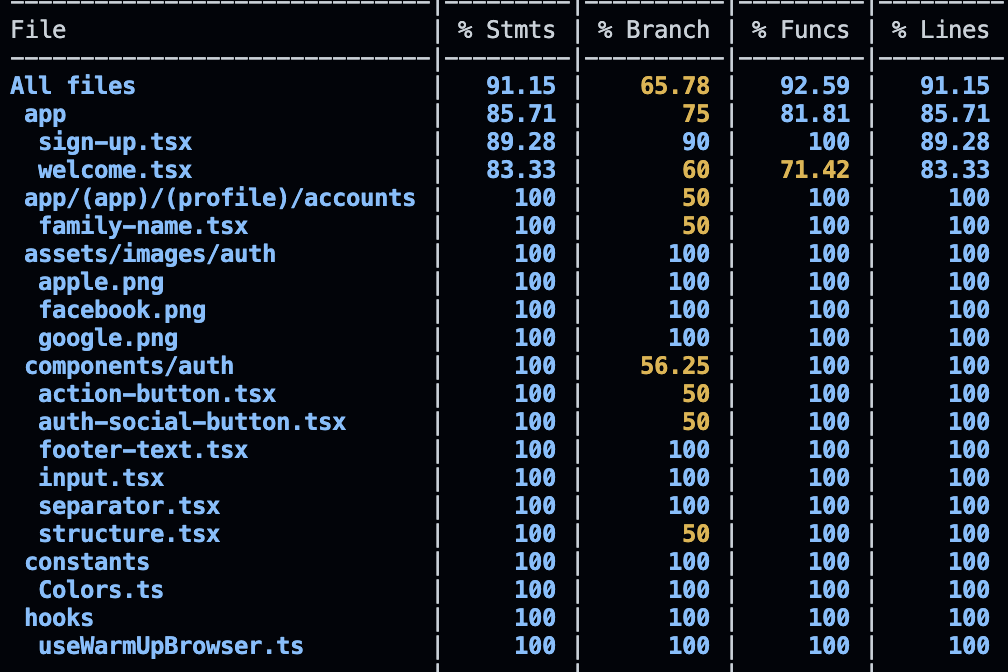
\includegraphics[width=1\linewidth, height=0.4\textheight]{Images/Coverage Report.png}
    \caption{Test Coverage Report}
\end{figure}


The above table shows the coverage for each file, indicating the percentage of statements, branches, functions, and lines that are covered by tests. \\\\
We followed the same process unless every component was tested and the coverage was above 80\% for all the components.

\vspace{1cm}

\textbf{Here is our Final Test coverage report results for all the components :}

\begin{figure}[H]
    \centering
    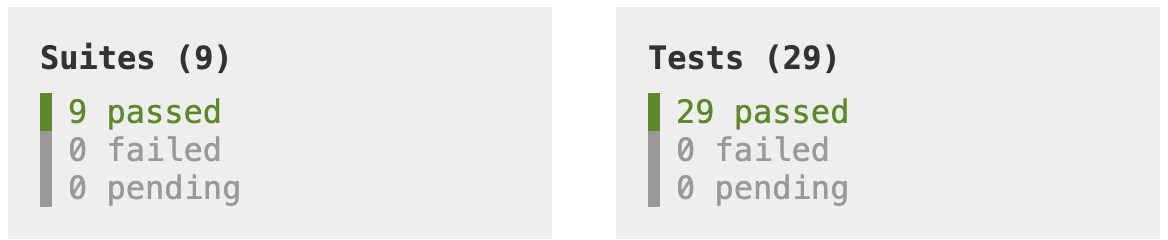
\includegraphics[width=1\linewidth, height=0.15\textheight]{Images/Test Results.png}
    \caption{Test Coverage Report}
\end{figure}

\textbf{Few examples of how we tested and what parts: }

\begin{figure}[H]
    \centering
    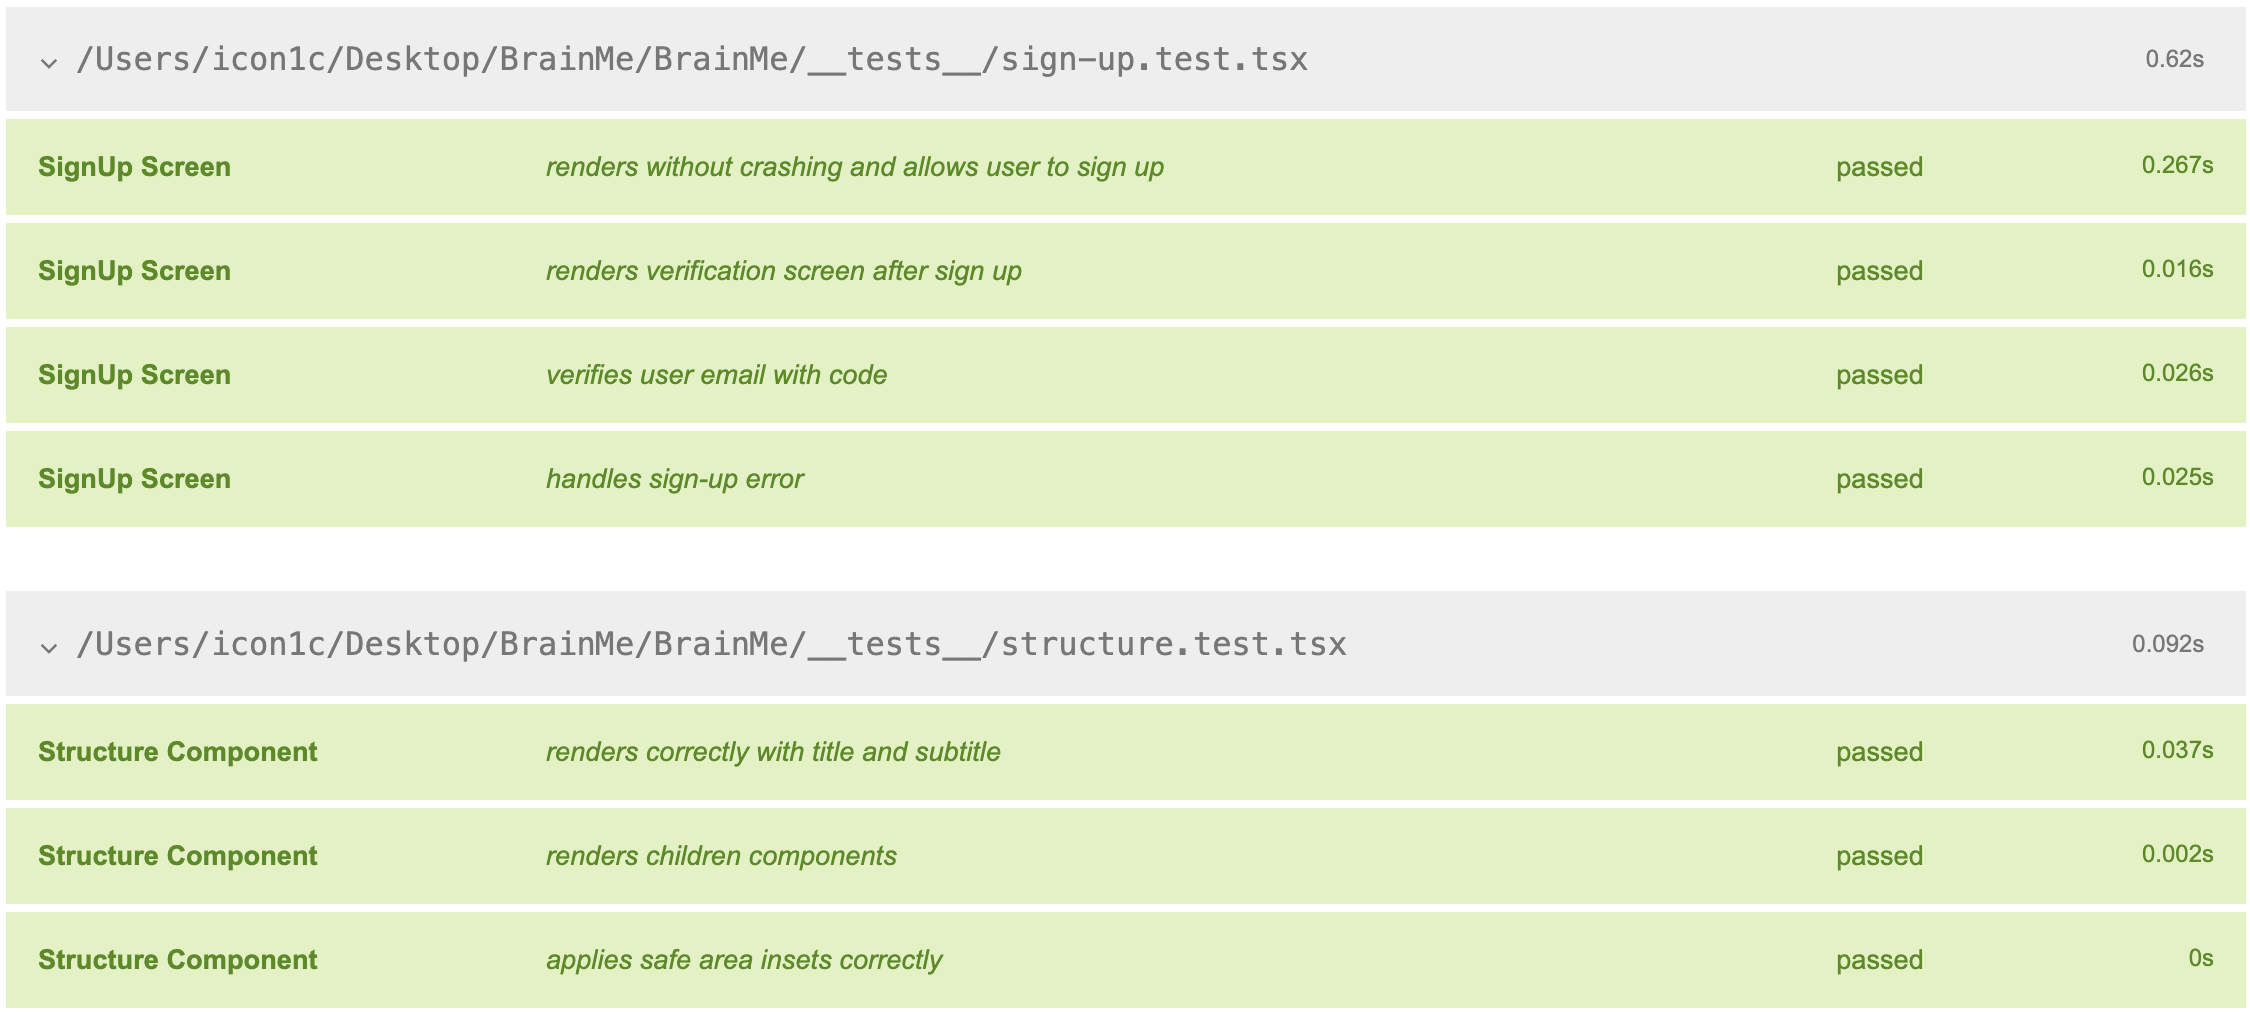
\includegraphics[width=1\linewidth, height=0.4\textheight]{Images/Test Results Example.png}
    \caption{Test Coverage Examples}
\end{figure}

By following these detailed steps in our testing campaign, we ensured that the BrainMe application is robust, reliable, and user-friendly.

\subsection{Automatic Testing}

We performed automatic testing to ensure that the BrainMe application functions correctly without manual intervention. Our goal was to achieve at least 80\% coverage. Automatic testing helped us quickly identify and fix issues, saving time and improving the reliability of the application.

\subsubsection{Goal of Automatic Testing}

The main goal of automatic testing was to validate that all parts of the application work as expected when executed automatically. We focused on:
\begin{itemize}
    \item Ensuring consistent and repeatable tests.
    \item Identifying defects quickly.
    \item Reducing the time and effort required for manual testing.
\end{itemize}

\subsubsection{Steps We Followed}

\begin{enumerate}
    \item \textbf{Select Testing Framework}: We chose Detox for end-to-end testing of our React Native application.
    \item \textbf{Write Test Scripts}: We wrote test scripts in TypeScript for various components of the application.
    \item \textbf{Set Up Test Environment}: We set up an environment where tests could run automatically.
    \item \textbf{Execute Tests}: We ran the test scripts automatically to check the functionality of different components.
    \item \textbf{Analyze Results}: We reviewed the test results to identify and fix any defects.
    \item \textbf{Repeat Tests}: We repeated the tests after fixing issues to ensure that the application works correctly.
\end{enumerate}

\subsubsection{Test Cases}

\begin{tabular}{|c|l|}
    \hline
    \textbf{Test Case ID} & \textbf{Description} \\
    \hline
    Test Case 1 & Automatically test the Login functionality. \\
    \hline
    Test Case 2 & Automatically test the Registration process. \\
    \hline
    Test Case 3 & Automatically test the Quiz feature. \\
    \hline
    Test Case 4 & Automatically test the Leaderboard functionality. \\
    \hline
    Test Case 5 & Automatically test the Profile management. \\
    \hline
    Test Case 6 & Automatically test the Settings adjustments. \\
    \hline
    Test Case 7 & Automatically test the overall user workflow from Login to Leaderboard. \\
    \hline
\end{tabular}

\vspace{1cm}

Each test case ensured that the specific components of the BrainMe application functioned correctly when tested automatically. By following this process, we efficiently identified and resolved issues, ensuring the application was reliable and user-friendly.

\subsubsection{Continuous Integration and Continuous Deployment (CI/CD)}

To streamline our development process, we integrated automatic testing with GitHub CI/CD. This ensured that our tests run every time we push code changes to the repository, helping us maintain code quality and reliability.

\begin{enumerate}
    \item \textbf{Set Up GitHub Actions}: We created a GitHub Actions workflow to automate the testing process.
    \item \textbf{Configure Workflow}: We configured the workflow to run Detox tests on every push and pull request.
    \item \textbf{Run Tests}: GitHub Actions automatically runs the tests and provides feedback on the test results.
    \item \textbf{Deploy on Success}: If all tests pass, the application is automatically deployed to the staging environment.
\end{enumerate}

\subsubsection{GitHub Actions Workflow}

Here is an example of the GitHub Actions workflow file we used:

\begin{verbatim}
name: CI/CD Pipeline

on: [push, pull_request]

jobs:
  build:
    runs-on: ubuntu-latest
    steps:
    - uses: actions/checkout@v2
    - name: Set up Node.js
      uses: actions/setup-node@v2
      with:
        node-version: '14'
    - name: Install dependencies
      run: npm install
    - name: Run tests
      run: npm test
    - name: Run Detox tests
      run: npm run test:detox
\end{verbatim}

This workflow checks out the code, sets up Node.js, installs dependencies, runs unit tests, and then runs Detox tests. If all tests pass, it proceeds to deployment. \\\\
By integrating automatic testing and CI/CD, we ensured that the BrainMe application remains stable and reliable, providing a seamless experience for our users.


\subsubsection{Goal of Integration Testing}

The main goal of our integration testing was to validate the interactions between the individual modules and to ensure that they function correctly when combined. We focused on:
\begin{itemize}
\item Ensuring that data flows correctly between modules.
\item Identifying and resolving interface defects.
\item Verifying that the integrated system meets the specified requirements.
\end{itemize}

\subsubsection{Steps We Followed}

\begin{enumerate}
\item \textbf{Identify Top-Level Components}: We started with the top-level component of the BrainMe application.
\item \textbf{Prepare Stubs for Lower-Level Components}: We created stubs for lower-level components that were not yet integrated.
\item \textbf{Develop Test Cases}: We wrote test cases to check the interactions between components.
\item \textbf{Execute Tests}: We integrated the top-level component with the stubs and ran the test cases.
\item \textbf{Integrate Lower-Level Components}: We replaced the stubs with actual lower-level components incrementally and continued testing.
\item \textbf{Repeat Until All Components are Integrated}: We continued this process until all components were integrated and tested.
\item \textbf{Validate Overall System Functionality}: We performed comprehensive testing to ensure that all components interact correctly and the overall system functions as expected.
\end{enumerate}

\subsubsection{Test Cases}

\begin{longtable}{|c|p{10cm}|}
\hline
\textbf{Test Case ID} & \textbf{Description} \\
\hline
Test Case 1 & Verify the functionality of the Login component with stubs for Registration and Dashboard. \\
\hline
Test Case 2 & Verify the functionality of the Login and Registration components with stubs for Quiz and Leaderboard. \\
\hline
Test Case 3 & Verify the functionality of Login, Registration, and Quiz components with stubs for Leaderboard and Profile. \\
\hline
Test Case 4 & Verify the functionality of Login, Registration, Quiz, and Leaderboard components with stubs for Profile and Settings. \\
\hline
Test Case 5 & Verify the functionality of Login, Registration, and Dashboard with stubs for Quiz and Settings. \\
\hline
Test Case 6 & Verify the functionality of Login, Registration, Dashboard, and Quiz components with stubs for Profile and Settings. \\
\hline
Test Case 7 & Verify the functionality of Login, Registration, Dashboard, Quiz, Profile, and Settings components. \\
\hline
\end{longtable}

Each test case ensured that the integrated components interacted correctly and met the expected requirements. Through this rigorous testing process, we achieved our goal of ensuring that the BrainMe application functions seamlessly as a cohesive system.

\subsection{User Test}

We conducted user tests with eight participants from diverse backgrounds to gather feedback on BrainMe. Each participant tested the application from installation to the leaderboard and provided detailed feedback on their experiences. Here are the results:

\subsubsection{Chiara Bottazzini: Bocconi Student, 24y, Female, Economics (CEMS)}

\begin{itemize}
    \item \textbf{Installation:} Chiara found the installation process smooth and straightforward. She appreciated the clear instructions provided.
    \item \textbf{Login and Registration:} She easily registered using her email and was able to log in without any issues. 
    \item \textbf{Quiz Experience:} Chiara enjoyed the quiz topics related to economics. She found the questions challenging but fair. 
    \item \textbf{Leaderboard:} The leaderboard was motivating for her. She liked seeing her rank compared to her peers.
    \item \textbf{Feedback:} Chiara mentioned that the user interface could be improved for better visual appeal. She also suggested adding more quiz topics related to her field.
\end{itemize}

\subsubsection{Thibault Beineix: HEC Student, 26, Male, Entrepreneurship}

\begin{itemize}
    \item \textbf{Installation:} Thibault found the app easy to download and install. The process was quick and hassle-free.
    \item \textbf{Login and Registration:} He registered using his email but faced a slight delay during the verification process.
    \item \textbf{Quiz Experience:} Thibault enjoyed the entrepreneurship quizzes. He found the questions engaging and relevant to his studies.
    \item \textbf{Leaderboard:} The leaderboard feature was exciting for him. It encouraged him to participate more actively.
    \item \textbf{Feedback:} Thibault suggested improving the speed of the email verification process. He also recommended adding more interactive elements in the quizzes.
\end{itemize}

\subsubsection{Maxime Limagne: EasyJet Pilot Student, 25, Male, Pilot Apprentice}

\begin{itemize}
    \item \textbf{Installation:} Maxime experienced a seamless installation process with no issues.
    \item \textbf{Login and Registration:} He registered quickly using his email and appreciated the straightforward process.
    \item \textbf{Quiz Experience:} Maxime did not find the aviation-related quizzes very strange. He enjoyed testing his knowledge in other fields field.
    \item \textbf{Leaderboard:} The leaderboard was a great addition for him, as it added a competitive edge to his learning.
    \item \textbf{Feedback:} Maxime suggested adding more aviation-specific content. He also mentioned that the app could benefit from a darker theme option for night use.
\end{itemize}

\subsubsection{Solène Marache: Bocconi Student, 26, Female, Economics (CEMS)}

\begin{itemize}
    \item \textbf{Installation:} Solène found the installation process easy and user-friendly.
    \item \textbf{Login and Registration:} She registered without any problems and found the login process smooth.
    \item \textbf{Quiz Experience:} Solène appreciated the variety of quiz topics available. She found the questions well-structured and informative.
    \item \textbf{Leaderboard:} The leaderboard was motivating for her, and she liked the idea of competing with friends.
    \item \textbf{Feedback:} Solène suggested adding more detailed explanations for quiz answers. She also recommended improving the app's speed during peak usage times.
\end{itemize}

\subsubsection{Romain Lafrance: Bocconi Student, 26, Male, Economics (CEMS)}

\begin{itemize}
    \item \textbf{Installation:} Romain had no issues with the installation process and found it quick.
    \item \textbf{Login and Registration:} He registered easily but felt the password requirements were a bit too strict.
    \item \textbf{Quiz Experience:} Romain enjoyed the quizzes but he particularly did not find those related to economics. He found the rest challenging and educational.
    \item \textbf{Leaderboard:} The leaderboard was a great motivator for him. He liked seeing his progress compared to others.
    \item \textbf{Feedback:} Romain suggested relaxing the password requirements slightly. He also recommended adding more interactive elements to the quizzes.
\end{itemize}

\subsubsection{Luigi d’Andria: Luiss School Student, 24, Male, HR Department}

\begin{itemize}
    \item \textbf{Installation:} Luigi found the installation process straightforward and efficient.
    \item \textbf{Login and Registration:} He registered quickly and appreciated the clear instructions provided.
    \item \textbf{Quiz Experience:} Luigi did not find HR-related quizzes. He found the remaining topics to be challenging and informative He found the questions relevant and well-formulated.
    \item \textbf{Leaderboard:} The leaderboard feature was motivating for him. He liked the competitive aspect it added.
    \item \textbf{Feedback:} Luigi suggested adding more HR-specific content. He also mentioned that the app could benefit from a more modern design.
\end{itemize}

\subsubsection{Dario Bagnoli: Luiss School Student, 26, Male, HR Department}

\begin{itemize}
    \item \textbf{Installation:} Dario experienced a smooth installation process with no issues.
    \item \textbf{Login and Registration:} He registered without any problems and found the login process straightforward.
    \item \textbf{Quiz Experience:} Dario did not find HR-related quizzes. He found the remaining topics to be challenging and informative.
    \item \textbf{Leaderboard:} The leaderboard was motivating for him, and he liked competing with his peers.
    \item \textbf{Feedback:} Dario suggested adding more detailed explanations for quiz answers. He also recommended improving the app’s speed during peak usage times.
\end{itemize}

\subsubsection{Adrian Valica: EPFL, 20, Male, Computer Science Student}

\begin{itemize}
    \item \textbf{Installation:} Adrian found the installation process easy and quick.
    \item \textbf{Login and Registration:} He registered using his email and appreciated the smooth process.
    \item \textbf{Quiz Experience:} Adrian enjoyed the computer science quizzes. He found the questions challenging and relevant to his studies.
    \item \textbf{Leaderboard:} The leaderboard feature was exciting for him. It encouraged him to participate more actively.
    \item \textbf{Feedback:} Adrian suggested adding more advanced computer science topics. He also recommended enhancing the app’s design for better user experience.
\end{itemize}
